%# -*- coding: utf-8 -*-
%!TEX encoding = UTF-8 Unicode
%!TEX TS-program = xelatex
% vim:ts=4:sw=4
%
% 以上设定默认使用 XeLaTex 编译,并指定 Unicode 编码,供 TeXShop 自动识别

%第六十回 
\chapter{李瓶兒病纏死孽 西門慶官作生涯}

詞曰:

倦睡懨懨生怕起,如痴如醉如慵,半垂半捲舊簾櫳。眼穿芳草綠,淚襯落花紅。
追憶當年魂夢斷,為雲為雨為風。凄凄樓上數歸鴻。悲淚三兩陣,哀緒萬千重。

話說潘金蓮見孩子沒了,每日抖擻精神,百般稱快,指著丫頭罵道:「賊淫婦!我只說你日頭常響午,卻怎的今日也有錯了的時節?你斑鳩跌了蛋──也嘴答谷了。春凳折了靠背兒──沒的椅了。王婆子賣了磨──推不的了。老鴇子死了粉頭──沒指望了。卻怎的也和我一般!」李瓶兒這邊屋裡分明聽見,不敢聲言,背地裡只是掉淚。著了這暗氣暗惱,又加之煩惱憂戚,漸漸精神恍亂,夢魂顛倒,每日茶飯都減少了。自從葬了官哥兒第二日,吳銀兒就家去了。老馮領了個十三歲的丫頭來,五兩銀子賣與孫雪娥房中使喚,改名翠兒,不在話下。

這李瓶兒一者思念孩兒,二者著了重氣,把舊病又發起來,照舊下邊經水淋漓不止。西門慶請任醫官來看,討將藥來吃下去,如水澆石一般,越吃越旺。那消半月之間,漸漸容顏頓減,肌膚消瘦,而精彩豐標無復昔時之態矣。正是:肌骨大都無一把,如何禁架許多愁!一日,九月初旬,天氣凄涼,金風漸漸。李瓶兒夜間獨宿房中,銀床枕冷,紗窗月浸,不覺思想孩兒,唏噓長嘆,恍恍然恰似有人彈的窗欞響。李瓶兒呼喚丫鬢,都睡熟了不答,乃自下床來,倒趿弓鞋,翻披繡襖,開了房門。出戶視之,彷彿見花子虛抱著官哥兒叫他,新尋了房兒,同去居住。李瓶兒還舍不的西門慶,不肯去,雙手就抱那孩兒,被花子虛只一推,跌倒在地。撒手驚覺,卻是南柯一夢。嚇了一身冷汗,嗚嗚咽咽,只哭到天明。正是:

有情豈不等,著相自家迷。

有詩為證:

纖纖新月照銀屏,人在幽閨欲斷魂。
益悔風流多不足,須知恩愛是愁根。

那時,來保南京貨船又到了,使了後生王顯上來取車稅銀兩。西門慶這裡寫書,差榮海拿一百兩銀子,又具羊酒金緞禮物謝主事:「就說此貨過稅,還望青目一二。」家中收拾鋪面完備,又擇九月初四日開張,就是那日卸貨,連行李共裝二十大車。那日,親朋遞果盒掛紅者約有三十多人,夏提刑也差人送禮花紅來。喬大戶叫了十二名吹打的樂工、雜耍撮弄。西門慶這裡,李銘、吳惠、鄭春三個小優兒彈唱。甘伙計與韓伙計都在柜上發賣,一個看銀子,一個講說價錢,崔本專管收生活。西門慶穿大紅,冠帶著,燒罷紙,各親友遞果盒把盞畢,後邊廳上安放十五張桌席,五果五菜、三湯五割,從新遞酒上坐,鼓樂喧天。在坐者有喬大戶、吳大舅、吳二舅、花大舅、沈姨夫、韓姨夫、吳道官、倪秀才、溫葵軒、應伯爵、謝希大、常峙節,還有李智、黃四、傅自新等眾伙計主管並街坊鄰舍,都坐滿了席面。三個小優兒在席前唱了一套《南呂•紅衲襖》「混元初生太極」。須臾,酒過五巡,食割三道,下邊樂工吹打彈唱,雜耍百戲過去,席上觥籌交錯。應伯爵、謝希大飛起大鐘來,杯來盞去。

飲至日落時分,把眾人打發散了,西門慶只留下吳大舅、沈姨夫、韓姨夫、溫葵軒、應伯爵、謝希大,從新擺上桌席留後坐。那日新開張,伙計攢帳,就賣了五百餘兩銀子。西門慶滿心歡喜,晚夕收了鋪面,把甘伙計、韓伙計、傅伙計、崔本、賁四連陳敬濟都邀來,到席上飲酒。吹打良久,把吹打樂工也打發去了,止留下三個小優兒在席前唱。

應伯爵吃的已醉上來,走出前邊解手,叫過李銘問道:「那個扎包髻兒清俊的小優兒,是誰家的?」李銘道:「二爹原來不知道?」因說道:「他是鄭奉的兄弟鄭春。前日爹在他家吃酒,請了他姐姐愛月兒了。」伯爵道:「真個?怪道前日上紙送殯都有他。」於是歸到酒席上,向西門慶道:「哥,你又恭喜,又抬了小舅子了。」西門慶笑道:「怪狗才,休要胡說。」一面叫過王經來:「斟與你應二爹一大杯酒。」伯爵向吳大舅說道:「老舅,你怎麼說?這鐘罰的我沒名。」西門慶道:「我罰你這狗才一個出位妄言。」伯爵低頭想了想兒,呵呵笑了,道:「不打緊處,等我吃,我吃死不了人。」又道:「我從來吃不得啞酒,你叫鄭春上來唱個兒我聽,我才罷了。」當下,三個小優一齊上來彈唱。伯爵令李銘、吳惠下去:「不要你兩個。我只要鄭春單彈著箏兒,只唱個小小曲兒我下酒罷。」謝希大叫道: 「鄭春你過來,依著你應二爹唱個罷。」西門慶道:「和花子講過:有一個曲兒吃一鐘酒。」叫玳安取了兩個大銀鐘放在應二面前。那鄭春款按銀箏,低低唱《清江引》道:

一個姐兒十六七,見一對蝴蝶戲。香肩靠粉牆,春筍彈珠淚。喚梅香趕他去別處飛。

鄭春唱了請酒,伯爵才飲訖,玳安又連忙斟上。鄭春又唱:

轉過雕欄正見他,斜倚定荼蘼架;佯羞整鳳衩,不說昨宵話,笑吟吟掐將花片兒打。

伯爵吃過,連忙推與謝希大,說道:「罷,我是成不的,成不的!這兩大鐘把我就打發了。」謝希大道:「傻花子,你吃不得推與我來,我是你家有
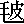
\includegraphics{figures-char/image00570.jpeg}%【毛皮】
的蠻子?」伯爵道:「傻花子,我明日就做了堂上官兒,少不的是你替。」西門慶道:「你這狗才,到明日只好做個韶武。」伯爵笑道:「傻孩兒,我做了韶武,把堂上讓與你就是了。」西門慶笑令玳安兒:「拿磕瓜來打這賊花子!」謝希大悄悄向他頭上打了一個響瓜兒,說道:「你這花子,溫老先生在這裡,你口裡只恁胡說。」 伯爵道:「溫老先兒他斯文人,不管這閑事。」溫秀才道:「二公與我這東君老先生,原來這等厚。酒席中間,誠然不如此也不樂。悅在心,樂主發散在外,自不覺手之舞之,足之蹈之如此。」

沈姨夫向西門慶說:「姨夫,不是這等。請大舅上席,還行個令兒──或擲骰,或猜枚,或看牌,不拘詩詞歌賦、頂真續麻、急口令,說不過來吃酒。這個庶幾均勻,彼此不亂。」西門慶道:「姨夫說的是。」先斟了一杯,與吳大舅起令。吳大舅拿起骰盆兒來說道:「列位,我行一令:順著數去,遇點要個花名,花名下要頂真,不拘詩詞歌賦說一句。說不來,罰一大杯。我就是一起──一擲一點紅,紅梅花對白梅花。」

吳大舅擲了個二,多一杯。飲過酒,該沈姨夫接擲。沈姨夫說道:

「二擲並頭蓮,蓮漪戲彩鴛。」

沈姨夫也擲了個二,飲過兩杯,就過盆與韓姨夫行令。韓姨夫說道:

「三擲三春李,李下不整冠。」

韓姨夫擲完,吃了酒,送與溫秀才。秀才道:「我學生奉令了──四擲狀元紅,紅紫不以為褻服。」

溫秀才只遇了一杯酒,吃過,該應伯爵行令。伯爵道:「我在下一個字也不識,不會頂真,只說個急口令兒罷:一個急急腳腳的老小,左手拿著一個黃豆巴鬥,右手拿著一條綿花叉口,望前只管跑走。一個黃白花狗,咬著那綿花叉口,那急急腳腳的老小,放下那左手提的那黃豆巴鬥,走向前去打那黃白花狗。不知手鬥過那狗,狗鬥過那手。」

西門慶笑罵道:「你這賊謅斷腸子的天殺的,誰家一個手去逗狗來?一口不被那狗咬了?」伯爵道:「誰叫他不拿個棍兒來!我如今抄化子不見了拐棒兒──受狗的氣了。」謝希大道:「大官人,你看花子自家倒了架,說他是花子。」西門慶道:「該罰他一鐘,不成個令。謝子純,你行罷!」謝希大道:「我也說一個,比他更妙:牆上一片破瓦,牆下一匹騾馬。落下破瓦,打著騾馬。不知是那破瓦打傷騾馬,不知是那騾馬踏碎了破瓦。」

伯爵道:「你笑話我的令不好,你這破瓦倒好?你家娘子兒劉大姐就是個騾馬,我就是個破瓦。──俺兩個破磨對瘸驢。」謝希大道:「你家那杜蠻婆老淫婦,撒把黑豆只好喂豬哄狗,也不要他。」兩個人鬥了回嘴,每人斟了一鐘,該韓伙計擲。韓道國道:「老爹在上,小人怎敢佔先?」西門慶道:「順著來,不要遜了。」於是韓道國說道:「五擲臘梅花,花里遇神仙。」

擲畢,該西門慶擲,西門慶道:「我要擲個六:六擲滿天星,星辰冷落碧潭水。」

果然擲出個六來。應伯爵看見,說道:「哥今年上冬,管情加官進祿,主有慶事。」於是斟了一大杯酒與西門慶。一面李銘等三個上來彈唱,頑耍至更闌方散。西門慶打發小優兒出門,看收了傢伙,派定韓道國、甘伙計、崔本、來保四人輪流上宿,吩咐仔細門戶,就過那邊去了。一宿晚景不題。

次日,應伯爵領了李智、黃四來交銀子,說:「此遭只關了一千四百五六十兩銀子,不夠還人,只挪了三百五十兩銀子與老爹。等下遭關出來再找完,不敢遲了。」 伯爵在旁又替他說了兩句美言。西門慶教陳敬濟來,把銀子兌收明白,打發去了。銀子還擺在桌上,西門慶因問伯爵道:「常二哥說他房子尋下了,前後四間,只要三十五兩銀子。他來對我說,正值小兒病重,我心裡亂,就打發他去了。不知他對你說來不曾?」伯爵道:「他對我說來,我說,你去的不是了,他乃郎不好,他自亂亂的,有甚麼心緒和你說話?你且休回那房主兒,等我見哥,替你題就是了。」西門慶道:「也罷,你吃了飯,拿一封五十兩銀子,今日是個好日子,替他把房子成了來罷。剩下的,叫常二哥門面開個小鋪兒,月間賺幾錢銀子兒,就夠他兩口兒盤攪了。」伯爵道:「此是哥下顧他了。」不一時,放桌兒擺上飯來,西門慶陪他吃了飯,道:「我不留你。你拿了這銀子去,替他乾乾這勾當去罷。」伯爵道:「你這裡還教個大官和我去。」西門慶道:「沒的扯淡,你袖了去就是了。」伯爵道:「不是這等說,今日我還有小事。實和哥說,家表弟杜三哥生日,早晨我送了些禮兒去,他使小廝來請我後晌坐坐。我不得來回你話,教個大官兒跟了去,成了房子,好教他來回你話的。」西門慶道:「若是恁說,叫王經跟你去罷。」一面叫王經跟伯爵來到了常家。

常峙節正在家,見伯爵至,讓進裡面坐。伯爵拿出銀子來與常峙節看,說:「大官人如此如此,教我同你今日成房子去,我又不得閑,杜三哥請我吃酒。我如今了畢你的事,我方纔得去。」常峙節連忙叫渾家快看茶來,說道:「哥的盛情,誰肯!」一面吃茶畢,叫了房中人來,同到新市街,兌與賣主銀子,寫立房契。伯爵吩咐與王經,歸家回西門慶話。剩的銀子,叫與常峙節收了。他便與常峙節作別,往杜家吃酒去了。西門慶看了文契,還使王經送與常二收了,不在話下。正是:

求人須求大丈夫,濟人須濟急時無。
一切萬般皆下品,誰知恩德是良圖。

